\subsection{One-Sided Limits, Monotone Functions, and Extended Limits}

\begin{definition} \label{def:one-sided-limits-and-discontinuities} \hlt{One-Sided Limits and Types of Discontinuity}\\
Let $X\subseteq\R$, $f:X\to\R$, and $x_0\in\R$.
\begin{enumerate}[label=(\roman*)]
\setlength{\itemsep}{0pt}
\item If $x_0$ is a limit point of $X\cap(x_0,\infty)$, then $f(x_0+)=q$ means $\lim\limits_{x\to x_0;\,x\in X\cap(x_0,\infty)}f(x)=q$.
\item If $x_0$ is a limit point of $X\cap(-\infty,x_0)$, then $f(x_0-)=q$ means $\lim\limits_{x\to x_0;\,x\in X\cap(-\infty,x_0)}f(x)=q$.
\item When $X$ approaches $x_0$ from both sides, the two-sided punctured limit through $X$ exists if and only if the two one-sided limits exist and are equal.
\end{enumerate}
For functions on an interval, a discontinuity with both one-sided limits is of the \hlt{first kind}, or \hlt{simple}; otherwise it is of the \hlt{second kind}. Simple discontinuities are jumps, $f(x_0+)\neq f(x_0-)$, or removable value mismatches.
\end{definition}

\begin{example} \label{ex:basic-discontinuity-types} \hlt{Basic Discontinuity Types}\\
Dirichlet's function $\mathbf{1}_{\Q}$ has a discontinuity of the second kind at every point.\\
The function $f(x)=x$ on $\Q$ and $f(x)=0$ off $\Q$ is continuous only at $0$; elsewhere its discontinuities are of the second kind. A jump in a piecewise linear function is a simple discontinuity.\\
Use Corollary \ref{cor:rationals-and-irrationals-dense}: every interval contains rational and irrational points.
\end{example}

\begin{figure}[H]
  \centering
  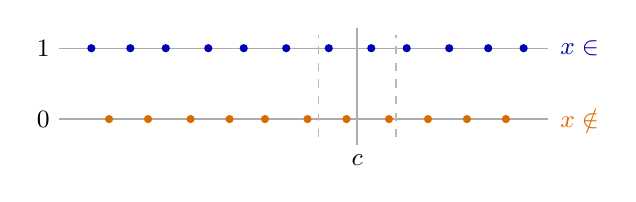
\begin{tikzpicture}[
  scale=0.90,
  every node/.style={font=\small},
  axis/.style={gray!65, line width=0.5pt},
  qdot/.style={circle, fill=blue!70!black, inner sep=1.05pt},
  idot/.style={circle, fill=orange!85!black, inner sep=1.05pt},
  window/.style={gray!55, dashed, line width=0.45pt}
]
  \draw[axis] (-3.45,1) -- (3.45,1);
  \draw[axis] (-3.45,0) -- (3.45,0);

  \foreach \x in {-3.0,-2.45,-1.95,-1.35,-0.85,-0.25,0.35,0.95,1.45,2.05,2.6,3.1} {
    \node[qdot] at (\x,1) {};
  }
  \foreach \x in {-2.75,-2.2,-1.6,-1.05,-0.55,0.05,0.6,1.2,1.75,2.3,2.85} {
    \node[idot] at (\x,0) {};
  }

  \coordinate (c) at (0.75,0);
  \draw[window] (0.20,-0.26) -- (0.20,1.18);
  \draw[window] (1.30,-0.26) -- (1.30,1.18);
  \draw[axis] (0.75,-0.36) -- (0.75,1.28);
  \node[below] at (0.75,-0.36) {$c$};

  \node[left] at (-3.45,1) {$1$};
  \node[left] at (-3.45,0) {$0$};
  \node[blue!70!black, right] at (3.48,1) {$x\in\Q$};
  \node[orange!85!black, right] at (3.48,0) {$x\notin\Q$};
\end{tikzpicture}

  \caption{For $g=\mathbf{1}_{\Q}$, interval around $c$ has rational inputs value $1$ and irrational inputs value $0$.}
  \label{fig:dirichlet-dense-rows}
\end{figure}

\begin{definition} \label{def:monotone-real-function} \hlt{Monotone Functions}\\
Let $f$ be real-valued on $(a,b)$. The function is \hlt{monotonically increasing} if $a<x<y<b$ implies $f(x)\leq f(y)$. Reversing the inequality gives \hlt{monotonically decreasing}. A \hlt{monotone} function is one of these two types.
\end{definition}

\begin{theorem} \label{thm:monotone-functions-one-sided-limits} \hlt{One-Sided Limits of Monotone Functions}\\
If $f$ is increasing on $(a,b)$, then for every $x\in(a,b)$, $\sup\limits_{a<t<x}f(t)=f(x-)\leq f(x)\leq f(x+)=\inf\limits_{x<t<b}f(t)$.\\
Moreover, $a<x<y<b$ implies $f(x+)\leq f(y-)$. For decreasing $f$, reverse the inequalities.
\begin{proof}
Let $A\defeq\sup_{a<t<x}f(t)$.\\
For every $\varepsilon>0$, choose $s<x$ with $A-\varepsilon<f(s)\leq A$; then $s<t<x$ implies $A-\varepsilon<f(t)\leq A$, so $f(x-)=A$.\\
Let $B\defeq\inf_{x<t<b}f(t)$. For every $\varepsilon>0$, choose $s>x$ with $B\leq f(s)<B+\varepsilon$; then $x<t<s$ implies $B\leq f(t)<B+\varepsilon$, so $f(x+)=B$. If $x<y$, then $\inf_{x<t<y}f(t)\leq\sup_{x<t<y}f(t)$ gives $f(x+)\leq f(y-)$.\\
For decreasing $f$, apply the increasing case to $-f$ and multiply the resulting inequalities by $-1$.\\
\hlt{Structural Commentary}: Monotonicity converts one-sided limits into suprema and infima.\\
\hlt{Key Insight}: A monotone function has jumps, but not oscillatory one-sided failure.
\end{proof}
\end{theorem}

\begin{corollary} \label{cor:monotone-no-second-kind-discontinuities} \hlt{Monotone Functions Have No Second-Kind Discontinuities}\\
A monotone real function on an interval has no discontinuities of the second kind.
\begin{proof}
At every interior point, Theorem \ref{thm:monotone-functions-one-sided-limits} gives both one-sided limits.\\
Hence any discontinuity is of the first kind by Definition \ref{def:one-sided-limits-and-discontinuities}.\\
\hlt{Structural Commentary}: Monotonicity rules out oscillatory discontinuities.\\
\hlt{Key Insight}: All monotone discontinuities are jumps or removable value mismatches.
\end{proof}
\end{corollary}

\begin{theorem} \label{thm:monotone-discontinuities-countable} \hlt{Monotone Discontinuities Are Countable}\\
If $f$ is monotone on $(a,b)$, then the set of points of $(a,b)$ at which $f$ is discontinuous is at most countable.
\begin{proof}
Assume $f$ is increasing, and let $E$ be its discontinuity set.\\
For each $x\in E$, Theorem \ref{thm:monotone-functions-one-sided-limits} gives $f(x-)<f(x+)$; choose $r(x)\in\Q$ with $f(x-)<r(x)<f(x+)$.\\
If $x_1<x_2$, then $f(x_1+)\leq f(x_2-)$, so $r(x_1)\neq r(x_2)$. Thus $E$ injects into $\Q$, hence is countable by Corollary \ref{cor:rationals-countable}. If $f$ is decreasing, apply the increasing case to $-f$, which has the same discontinuity set.\\
\hlt{Structural Commentary}: Each jump contains a rational marker, and monotonicity keeps the markers distinct.\\
\hlt{Key Insight}: Countability enters by injecting discontinuities into $\Q$.
\end{proof}
\end{theorem}

\begin{remark} \label{rem:monotone-discontinuities-need-not-be-isolated} \hlt{Monotone Discontinuities Need Not Be Isolated}\\
For countable $E=\{x_n:n\in\N\}\subset(a,b)$ and positive summable $(c_n)$, $f(x)=\sum\limits_{x_n<x}c_n$ is increasing, has jumps of size $c_n$ at $x_n$, and is continuous off $E$. Thus monotone discontinuities may be dense.
\end{remark}

\begin{definition} \label{def:extended-real-function-limits} \hlt{Extended Limits and Limits at Infinity}\\
Neighborhoods of $+\infty$ are intervals $(c,+\infty)$; neighborhoods of $-\infty$ are $(-\infty,c)$.\\
For $f:E\to\R$ and extended real $A,x$, $f(t)\to A$ as $t\to x$ means: every neighborhood $U$ of $A$ contains $f(t)$ for all punctured $t\in E$ sufficiently near $x$, i.e. $\exists V\ni x$ such that $t\in V\cap E,\ t\neq x$ $\Longrightarrow$ $f(t)\in U$.\\
For real $A,x$, this agrees with Definition \ref{def:function-limit-metric}.\\
\hlt{Structural Commentary}: Extended limits use same neighborhood test, $\pm\infty$ allowed as input or output limits.
\end{definition}

\begin{theorem} \label{thm:extended-limit-algebra} \hlt{Algebra of Extended Limits}\\
Let $f,g:E\to\R$ and $f(t)\to A$, $g(t)\to B$ as $t\to x$, with $A,B,x$ extended real. Then, whenever RHS is defined:
\begin{enumerate}[label=(\roman*)]
\setlength{\itemsep}{0pt}
\item if $f(t)\to A'$ as $t\to x$, then $A'=A$;
\item $(f+g)(t)\to A+B$;
\item $(fg)(t)\to AB$;
\item $(f/g)(t)\to A/B$;
\end{enumerate}
The forms $\infty-\infty$, $0\cdot\infty$, $\infty/\infty$, and $A/0$ are undefined.
\begin{proof}
\begin{enumerate}[label=(\roman*)]
\setlength{\itemsep}{0pt}
\item If $A'\neq A$, choose disjoint neighborhoods of $A$ and $A'$.\\
Definition \ref{def:extended-real-function-limits} would eventually place $f(t)$ in both, a contradiction.
\item For any neighborhood $W$ of $A+B$, definedness gives neighborhoods $U$ of $A$ and $V$ of $B$ such that $u+v\in W$ for $u\in U$, $v\in V$. Apply the two limits in a common punctured neighborhood of $x$.
\item The same neighborhood argument applies to multiplication, excluding $0\cdot\infty$.
\item Apply it to division; since $B\neq0$, choose the neighborhood of $B$ away from $0$.
\end{enumerate}
\hlt{Structural Commentary}: Extended limit algebra is ordinary limit algebra in neighborhood form.\\
\hlt{Key Insight}: The undefined forms are exactly where neighborhood control breaks.
\end{proof}
\end{theorem}
